\section{State of art}

In this section we deal with the current state of the art of process theory, simulation and visualization of elementary processes in the oxygen converter used in steelmaking. There have been tremendous improvements in iron and steelmaking processes in the past twenty years. Productivity and coke rates in the blast furnace and the ability to refine steel to demanding specifications have been improved significantly. Much of this improvement is based on the application of fundamental principles and thermodynamic and kinetic parameters which have been determined \citep{Turkdogan1999}.

\subsection{Process control}

The need for developing improved control systems has traditionally been powered by the demand for more accurate and cost efficient production. This is still a major driving force but environmental issues do also have a profound influence on this development today \citep{Widlund1998}.

The main objective of controlling oxygen converter steelmaking is to obtain prescribed parameters for the steel when it is tapped from the furnace, including weight, temperature, and each element content. In practical steelmaking process, the criterion whether the molten steel is acceptable or not is often decided by the endpoint carbon content and temperature \citep{Wang2010}.

The fast dynamics of the LD converter steelmaking process or the BOF process, as it is commonly known, often makes it a challenge to obtain stable blowing conditions and to achieve the required steel composition and temperature simultaneously at the end point. For this reason, process control becomes very necessary and attempts had started as early as in the 1970s \citep{Fritz2005}. Out of the originally very simple LD process have grown the modern process-controlled and automated production systems that enable present-day adaptations to meet today’s economic and ecological demands \citep{Sarkar2015}.

Generally, the BOF steelmaking process with sub-lance system can be divided into two stages: static control and dynamic control. Static models include oxygen supplying model, slaging model and bottom blowing model; dynamic models include decarburization speed model, molten steel warming model and the model for the amount of coolant. \citep{Wang2010}.


--------------------- okresat ------------------

Deviations from the desired process course can be caused by several factors. These factors may be described in four different categories; process, hardware, operator induced irregularities and production disturbances \citep{Widlund1998}.

Process irregularities. There is a contradiction between the need to obtain high slag levels to provide good refining conditions and the desire to minimise uncontrolled slag overflow, "slopping" . All events of slopping result in severe dust emissions and iron yield losses affecting the mass and heat balance computations by the control system. FW'thermore, production must be stopped to allow for cleaning of the vessel mouth and the area below the vessel \citep{Widlund1998}.

Unknown scrap dissolution rate may also interfere with process performance. Late melting of high-carbon scrap can cause uncertain composition of sample taken with a sub lance resulting in erratic feed-back to the control system \citep{Widlund1998}.

Hardware irregularities. Hot metal temperature measurements in the transfer ladle are made by means of a thennocouple and believed to be reliable. However, it remains unclear whether the measW'ement is representative for the total amount of the hot metal to be charged to the converter. Weighing equipment for hot metal, scrap and other additions is regularly calibrated but still has an insufficient accuracy. This influences the reliability of the model computations and estimations in the control system. The use of gas analysis in a control system is hindered by the presence of long time delays (up to 25 seconds) in the measuring system. Unknown and inconsistent wear of the fiunace lining as well as the lance nozzles will also introduce uncertainties in the control system since these parameters influence the iron oxidation \citep{Widlund1998}.

Operator induced irregularities. Most of the existing systems require control actions from the operator and therefore to some extent depend on the operator's experience and personal preferences. For instance, it is a common practice that operators add other material amotmts than those recommended by the control system. It is not uncommon that the pre-set lance programs are shifted up- or downwards according to the operator's interpretation of previous heats. Furthermore, since reliable real-time measurements of the carbon content are not presently available, different operators apply different rules for deciding when to stop the blow. These operator induced irregularities make it difficult to achieve Production disturbances. The converter process is only one link in a chain of unit operations from raw materials 10 fmal product. Therefore, production disturbances can change process conditions. For example, poor blast furnace performance might lead to insufficient hot metal supply or even production disruptions. Under these circumstances, more metal scrap and fuel should be used instead of hot metal to uphold production volumes. Logically, this implies changes in blowing practice \citep{Widlund1998}.

---------------------------------------

In order to monitor and/or control the process, different measuring systems can be employed to give feedback to either the operator or directly to existing system for automated control. These measurements can be either direct or indirect as well as with or without time delays \citep{Widlund1998}.

The real-time information on the process state can be obtained from a nwnber of sensors \citep{Widlund1998}.

Sensor: Flow rate measurement with venturi
Information obtained: Off-gas flow rate.
Sound level measurement with microphone
Indication of changes in slag level.
Load cell or accelerometer on lance or vessel
Indication of changes in slag level.
Temperature measurement Off-gas temperature. Lance elongation Hood pressure
Indication of changes in slag level. Pressure difference with ambient pressure.

All these signals can, in principle, be used for closed-loop control \citep{Widlund1998}.

There are only a few process variables that can be manipulated by the control system or the operator - lance height, oxygen gas flow rate and purge gas flow rate. Naturally, changes in lance height are easier to measure as well as set and therefore preferable to use in a closed- loop control system. Oxygen gas flow rate should not be changed more than approximately $\pm$5\% since the nozzle is designed for a specific flow rate \citep{Widlund1998}.

Two basic approaches to control the process are; open-loop control and closed-loop control. The former assumes availability of a pre-defined control signal trajectory bringing the process to a desired state. Using the latter, measurements of the process output signals are fed back to the actuators via a controller. An obvious shortcaning of the open-loop strategy is a high sensitivity to process disturbances. Thus, a closed-loop control system of the BOS converter is sought. A major difficulty in designing such a system would be the necessity to analyse stability and performance of the closed-loop system \citep{Widlund1998}.

\subsection{Computer-aided Mathematical Modeling and Numerical Simulation}

The motivation for using computer simulations to investigate metallurgical processes is two-fold. First, it enables design changes to be tested before building a prototype, which naturally leads to a lower total design cost. Second, it makes it possible to investigate phenomena that cannot easily be measured or observed in the process. Even a seemingly simple operation such as the continuous measurement of the temperature during the decarburization process is difficult due to the very high temperatures in the process and generally harsh conditions prevailing in the steel plants \citep{Ersson2018}.

In metallurgy, simulating linear and non-linear processes that we encounter in steelmaking by creating mathematical models is of great importance. Since first attempts to use mathematical techniques for the simulation and optimization of large scale metallurgical operations \citep{Ray1973}, various numerical methods were implemented as algorithms and used to simulate phenomena in steelmaking processes. One class of such methods is called Monte Carlo, which is useful for simulating systems with many coupled degrees of freedom such as fluids.

Modern fluid mechanics problems would be impossible to solve without use of Computational Fluid Dynamics (CFD), since the scope of analytical solutions to fundamental equations of fluid mechanics is very limited and, once a more difficult geometry is encountered, we usually have to choose a given numerical method
for obtaining a solution. CFD encompasses a wide spectrum of numerical methods used for solving complex three-dimensional (3D) and time-dependent flow problems \citep{RAPP20173}. Since early pioneering work in the metallurgical field done by \citet{Szekely1977}, the cost of performing computer simulations has decreased over the last few decades, while the available processing power has increased. Most of the processors and  processing units that are currently developed and produced have several cores that can execute instructions in parallel. Thus, the processing power available to a CFD software also depends on the capability of the software to execute in parallel. A study by \citet{Ersson2018} of the last two decades of metallurgical CFD simulations reveals huge improvements on the type of phenomena that can be explored and we will see this trend is continuing thanks to improvements in both the available processing power and the available algorithms. Therefore CFD found its way into numerous studies in steelmaking, where these methods proved useful in demonstrating the hidden and significant properties. However, its use in the steel industry may not be as integrated as in the aero and automotive industries, in which the development of new designs is of key importance. The major difference between aero and metallurgical industries is that the metallurgical industries almost always deal with multiphase systems at elevated temperatures and that the motivation of modeling is mainly process optimization. With a continuing development in multiphase models as well as in reacting flow modeling, the continued usefulness of CFD in metallurgy remains clear.

In LD/BOF process, different chemical reactions among oxygen, slag, and molten iron in oxygen converter, in combination with vigorous stirring process to promote slagging, dephosphorization, decarbonization, heating of molten steel, and homogenization of steel composition and temperature, determines the final properties of steel. The objective of the oxygen converter is to refine molten iron to crude steel through oxidization to achieve a specified temperature and chemical composition at the end blow. Failure to do this leads to the need to reblow. The impact of oxygen jet into molten bath strongly affects the bath and promotes the three-phase flow among gas, slag, and molten steel in the bath. With the move from old rule-based systems to a model-based, real-time closed-loop control of lance movement and oxygen flow, significant drawbacks were eliminated. There have been efforts in developing accurate and efficient numerical models within CFD field to solve the jets flow in the oxygen converter. \citet{Peng1996} established the conditions of optimum nozzles of performance by deriving the system of mathematical equations to simulate the steady, quasi-one-dimensional supersonic flow through a single De Laval nozzle. \citet{Tago2003} analyzed single-nozzle and multi-nozzle lances with the help of two-dimensional simulation based on fluid dynamics and found that higher ambient temperature leads to the lower density and the higher velocity of the gas jets, but does little affect the dynamic pressure. They report that CFD proved useful method to predict the effect of the inclination angle and the number of the nozzles on the jet behavior in the top blown processes. \citet{WangW2010} developed a three-dimensional mathematical model to simulate the compressible jets flow from the top-blown lance, taking into consideration variations of fluid density, viscosity, high temperature and Mach number. They demonstrated that $k–\omega$ turbulence model is superior to the widely used $k–\epsilon$ turbulence model to calculate turbulent conditions within multiple jets. Simulation results of final computational flow field distributions of three kinds of multiple jets are shown in Fig (\ref{o:m1}).

\begin{figure}[h!tbp]
	\centering
	\subfloat[Velocity magnitude (m/s)]{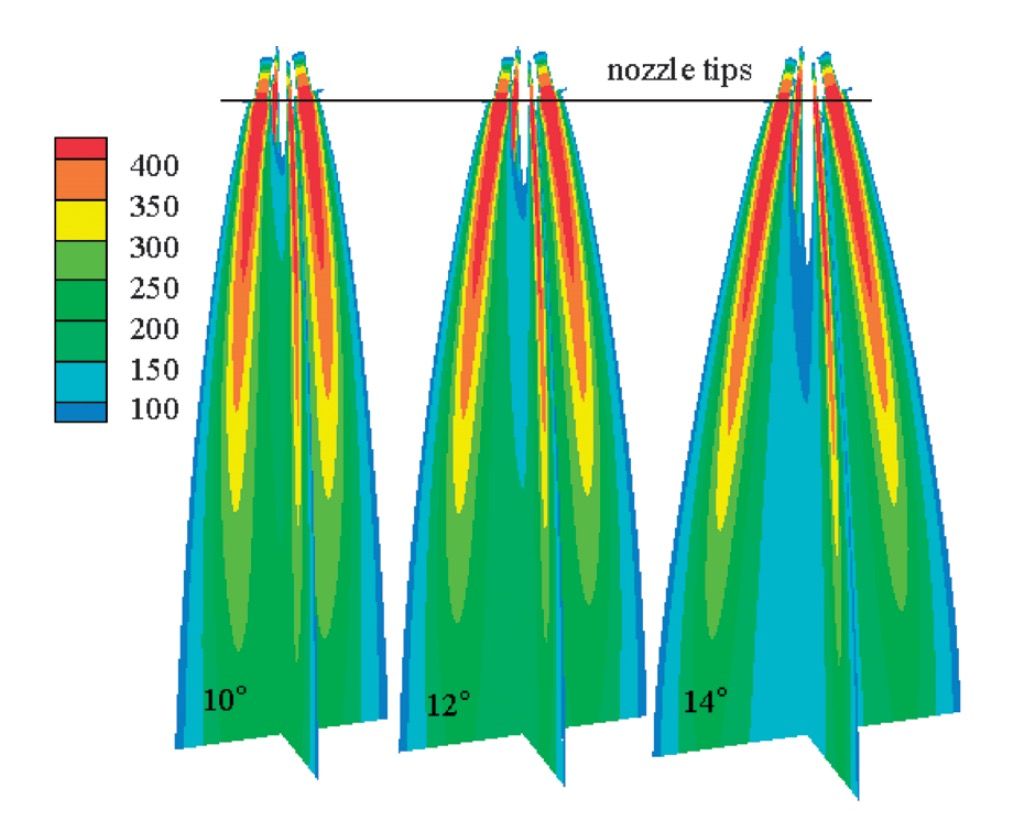
\includegraphics[width=0.6\textwidth]{cfd-velocity-magnitude.jpg}\label{fig:m1}}
	\hfill
	\subfloat[Total temperature (K)]{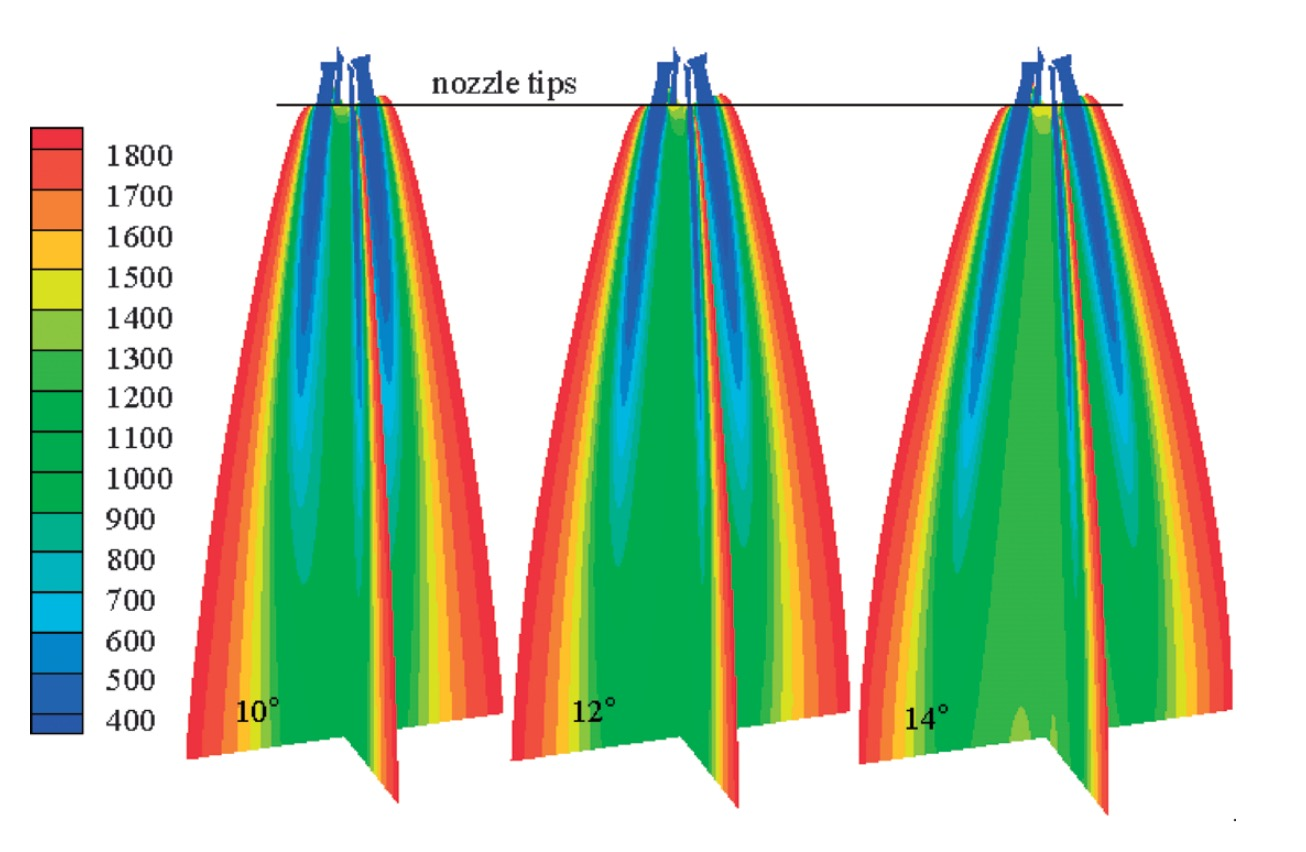
\includegraphics[width=0.7\textwidth]{cfd-total-temperature.jpg}\label{fig:m2}}
	\caption{Simulating results of velocity magnitude and total temperature field distributions of the three kinds of multiple jets: (a) velocity magnitude (m/s) and (b) total temperature (K) \citep{WangW2010}.}
	\label{o:m1}
\end{figure}

CFD models have been also used in developing deeper understanding of the decarburization processes in steelmaking. However, these processes are highly complex with large variations in time and length, and therefore it makes the systems extremely demanding to simulate. \citet{Ersson2018} reviewed latest research on the subject from 1998 until 2016 and found out that, even though several reports have been published discussing research about modeling parts of the decarburization processes numerically, no models have been presented that can handle the entire complexity of the processes. Many authors had simplified the system in existing models in order to achieve an understanding of particular phenomena rather than of the entire process.

Another important part of the oxygen steelmaking process is keeping the usual balance of 80\% hot metal and 20\% scrap during charging to regulate the temperature of steel in the vessel. To define the charge conditions and oxygen blowing requirements to achieve the temperature and chemical composition, mathematical and thermodynamic models have been developed \citep{Kacur2019,Sprava2018}. Reactions that take place in LD process can vary significantly from heat to heat, while not many variables involved are not accurately known. Therefore, it is necessary to take into account the uncertainty affecting the whole process reactions. To correct the differences between the theoretical predictions of the process models and the real results, \citet{Bouhouche2012} introduced a random quantity term into their models and improved the prediction model with the use of Support Vector Regression and Monte Carlo Simulation methods in combination. Most of the control schemes rely on an accurate system model. However, as these systems become more complex, writing down the dynamics from the first principles is extremely challenging. In such cases, neural networks are used to approximate the dynamics directly using system data. In this context, neural networks can be thought of as a generalization of linear regression for non-linear dynamics. At the Institute of Control and Informatization of Production Processes at BERG Faculty (TUKE), team around \citet{Sprava2018} built upon Bouhouche's work and started experimenting with machine learning in process control and its application in oxygen steelmaking, precisely in LD converter. They applied Support Vector Machines (SVM) and Support Vector Regression (SVR) to predict the final melt temperature and final carbon concentration based on dynamical data. Their work also focuses on developing innovative fractional-order mathematical models for indirect measurement of molten steel temperature and concentration of \ce{CO} and \ce{CO2}. The non-linear nature of these processes presents the opportunity to model them by using derivatives of non-integer order, which in their definition are based on the influence of past data on the present value of derivative.

Control of non-linear systems was the subject of intensive studies in the last few decades.


Fractional-order dynamic systems

fractional-order gradient method for backward propagation of neural networks \citep{Sheng2019}

\subsection{Visualization and Virtual Reality}

- O VRku
- Immersiveness, immersive, immersivity
- Non-immersive vs immersive

Scientific visualization is the use of computer graphics to create visual images that aid in the understanding of complex numerical representations of scientific concepts or results. As discussed in previous chapter, computational fluid dynamics (CFD) based numerical simulations often output massive amounts of data. These simulations often contain high-dimensional data in a three-dimensional volume. The display of phenomena associated with this data may involve complex three-dimensional structures.


 Such numerical representations, or data sets, may be the output of numerical simulations, as in computational fluid dynamics (CFD) or molecular modeling; recorded data, as in geological or astronomical applications; or constructed shapes, as in visualization of topological arguments. These simulations often contain high-dimensional data in a three- dimensional volume. The display of phenomena associated with this data may involve complex three- dimensional structures. Non-immersive interactive visualization systems implemented for the convention- al desktop and mouse are effective for moderately complex problems. Virtual reality displays aid in the unambiguous display of these structures by providing a rich set of spatial and depth cues. Virtual reality interface concepts allow the rapid and intuitive exploration of the volume containing the data, enabling the phenomena at various places in the volume to be explored, as well as provide simple control of the visualization environment through interfaces integrated into the environment \citep{Bryson1996}.

Luckily for many scientific visualization applications, the graphical rendering is to some extent arbitrary and can be chosen specifically to satisfy the perfor- mance constraints. This situation contrasts with the high-fidelity visual simulation of the real world, which can require time-consuming photo-realistic render- ing techniques. Consider again the example of streamlines in CFD. A streamline is simply an array of points in three dimensions. The array can be simply rendered as lines, allowing very fast rendering. This example can be generalized into a principle for developing real-time interactive visualization systems: Keep the graphical rendering as simple as possible \citep{Bryson1996}.

Beside mathematical modeling and simulations, creating a graphical representation of environments where particular processes happen is also very important and effective method when designing a future plant or planning upgrades to an already established one. It's important to understand the physical dimensions of  is  spatially explorable modelling of environment

\begin{figure}[h!]
	\centering
	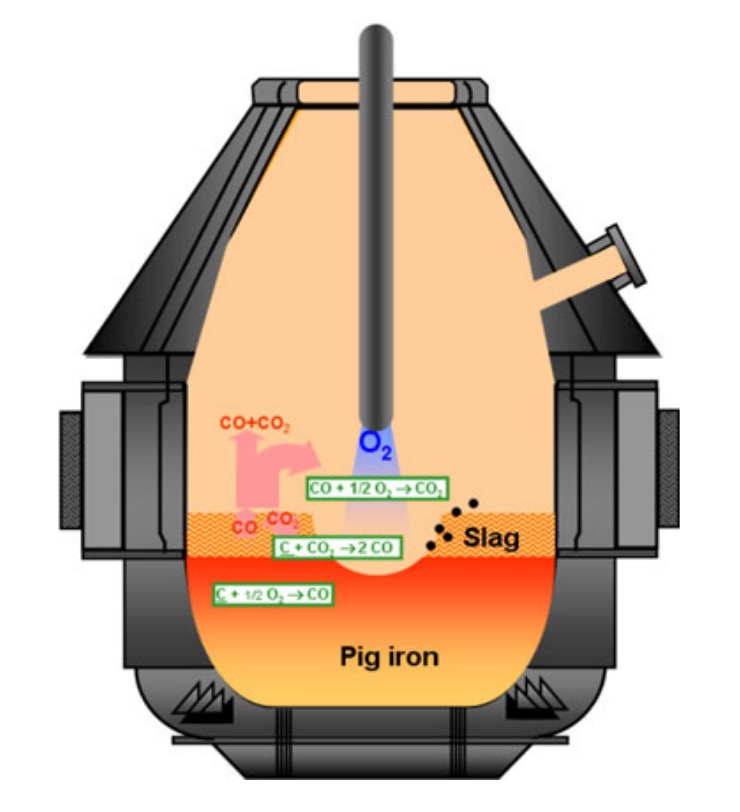
\includegraphics[width=.45\textwidth,angle=0]{bof-schematic.jpg}
	\caption{Static representation of basic oxygen furnace \citep{Doh2013}.}
	\label{o:m4}
\end{figure}

In some simplified form, the simulation of steelmaking processes can be used as a educational tool in process control courses at technical universities. The aim of the online, web-based interactive simulation of basic oxygen steelmaking at steeluniversity.org shown in Fig. \ref{o:m5} is to introduce students to this process in a more fun and engaging way.

\begin{figure}[h!]
	\centering
	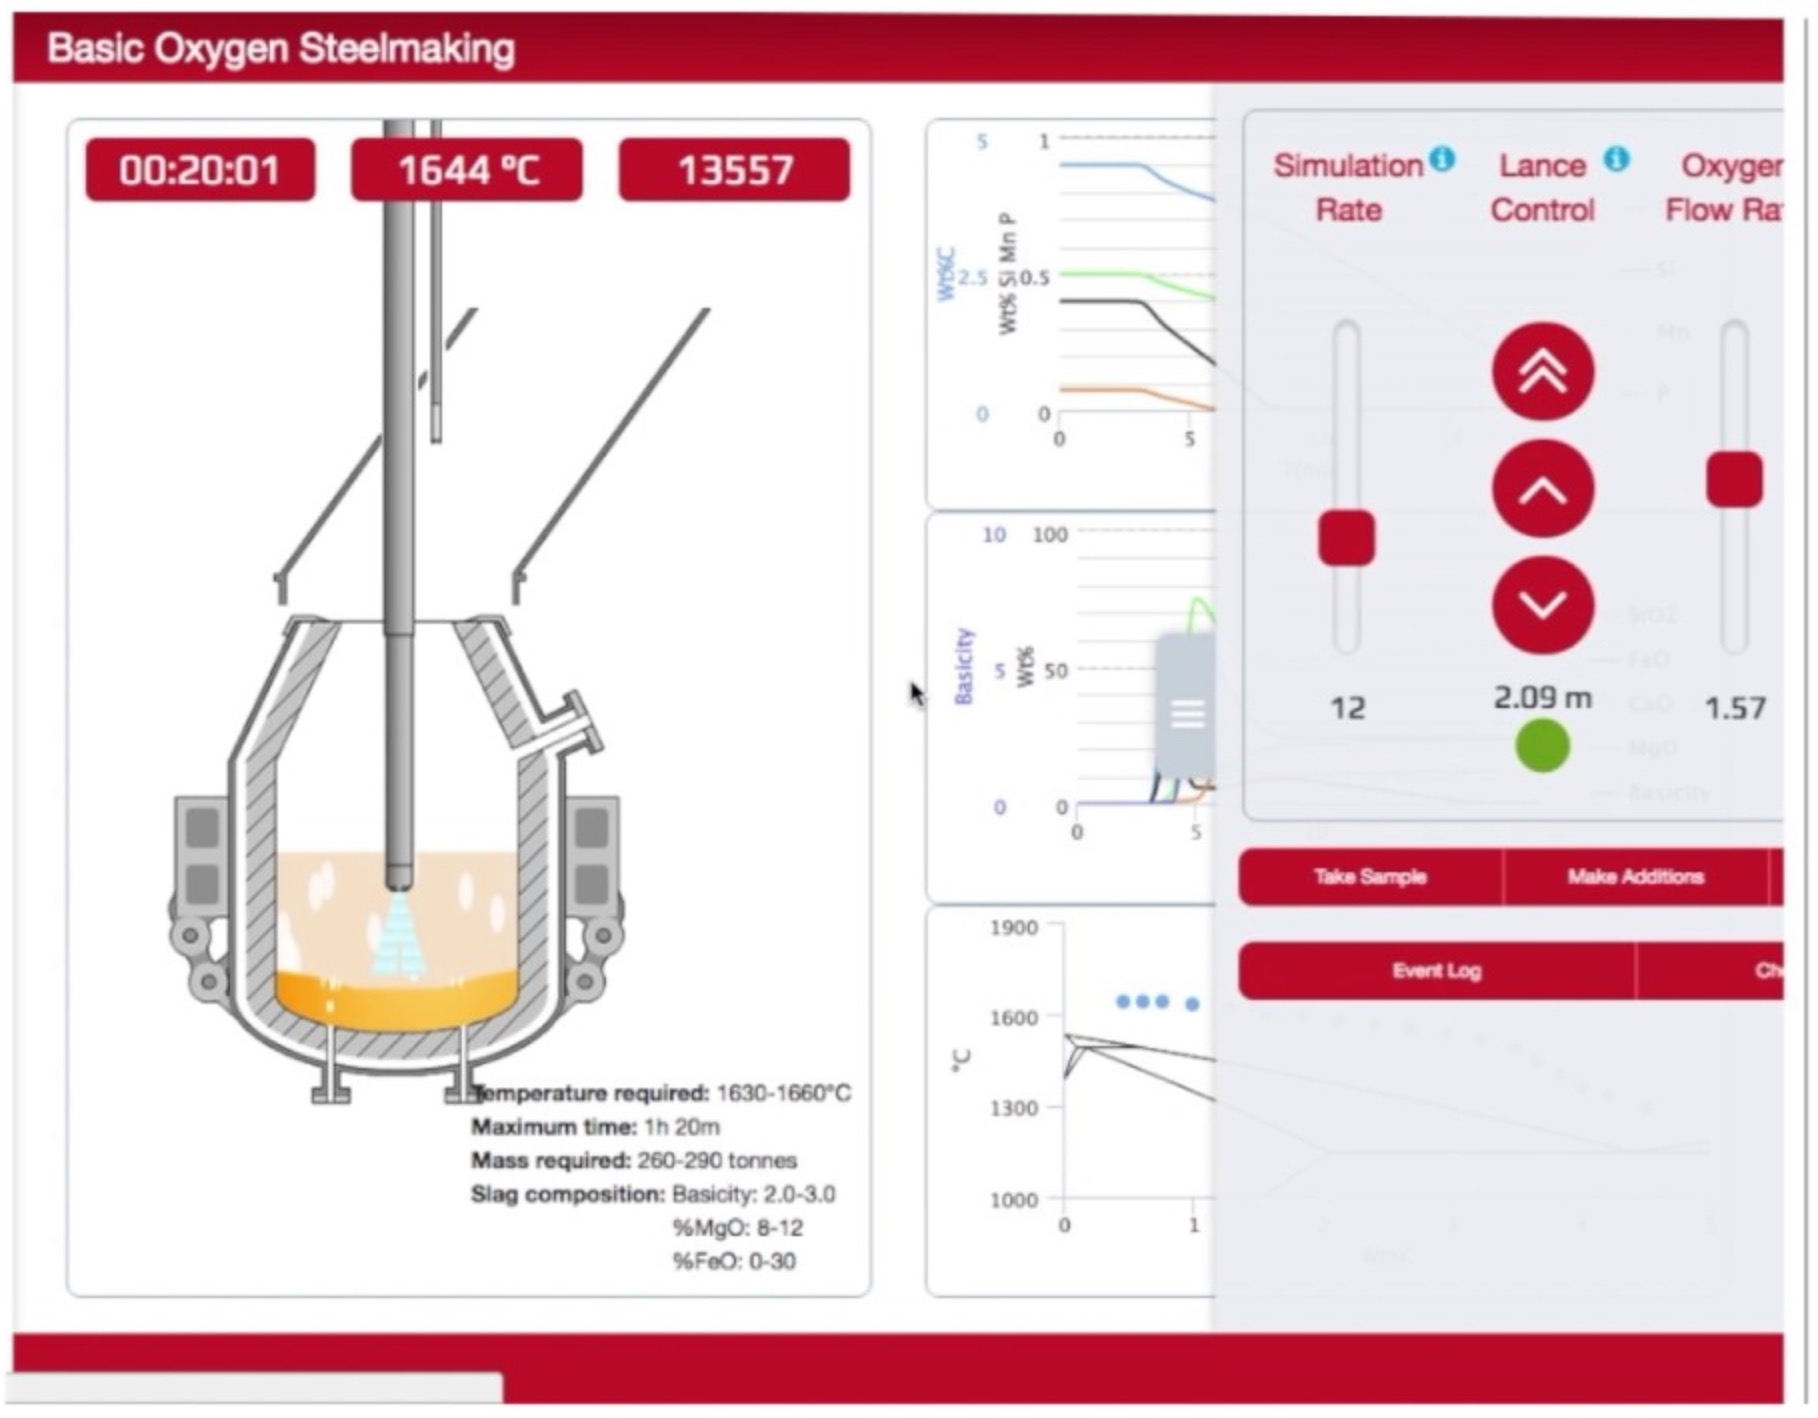
\includegraphics[width=.8\textwidth,angle=0]{steeluniversity.jpg}
	\caption{Interactive, educational simulation of basic oxygen steelmaking by steeluniversity.org.}
	\label{o:m5}
\end{figure}

A 3-D comprehensive CFD model has been developed, by \citet{Zheng2014} of Purdue University, specifically for simulating the blast furnace hearth. It includes both the hot metal flow and conjugate heat transfer through the refractories. The model has been extensively validated using measurement data from
industry blast furnace. Good agreements between measured and calculated refractory temperature profiles haven been achieved. The virtual reality (VR) visualization technology has been used to analyze the velocity and temperature distributions and wear patterns of different furnaces and operating conditions.

\begin{figure}[h!]
	\centering
	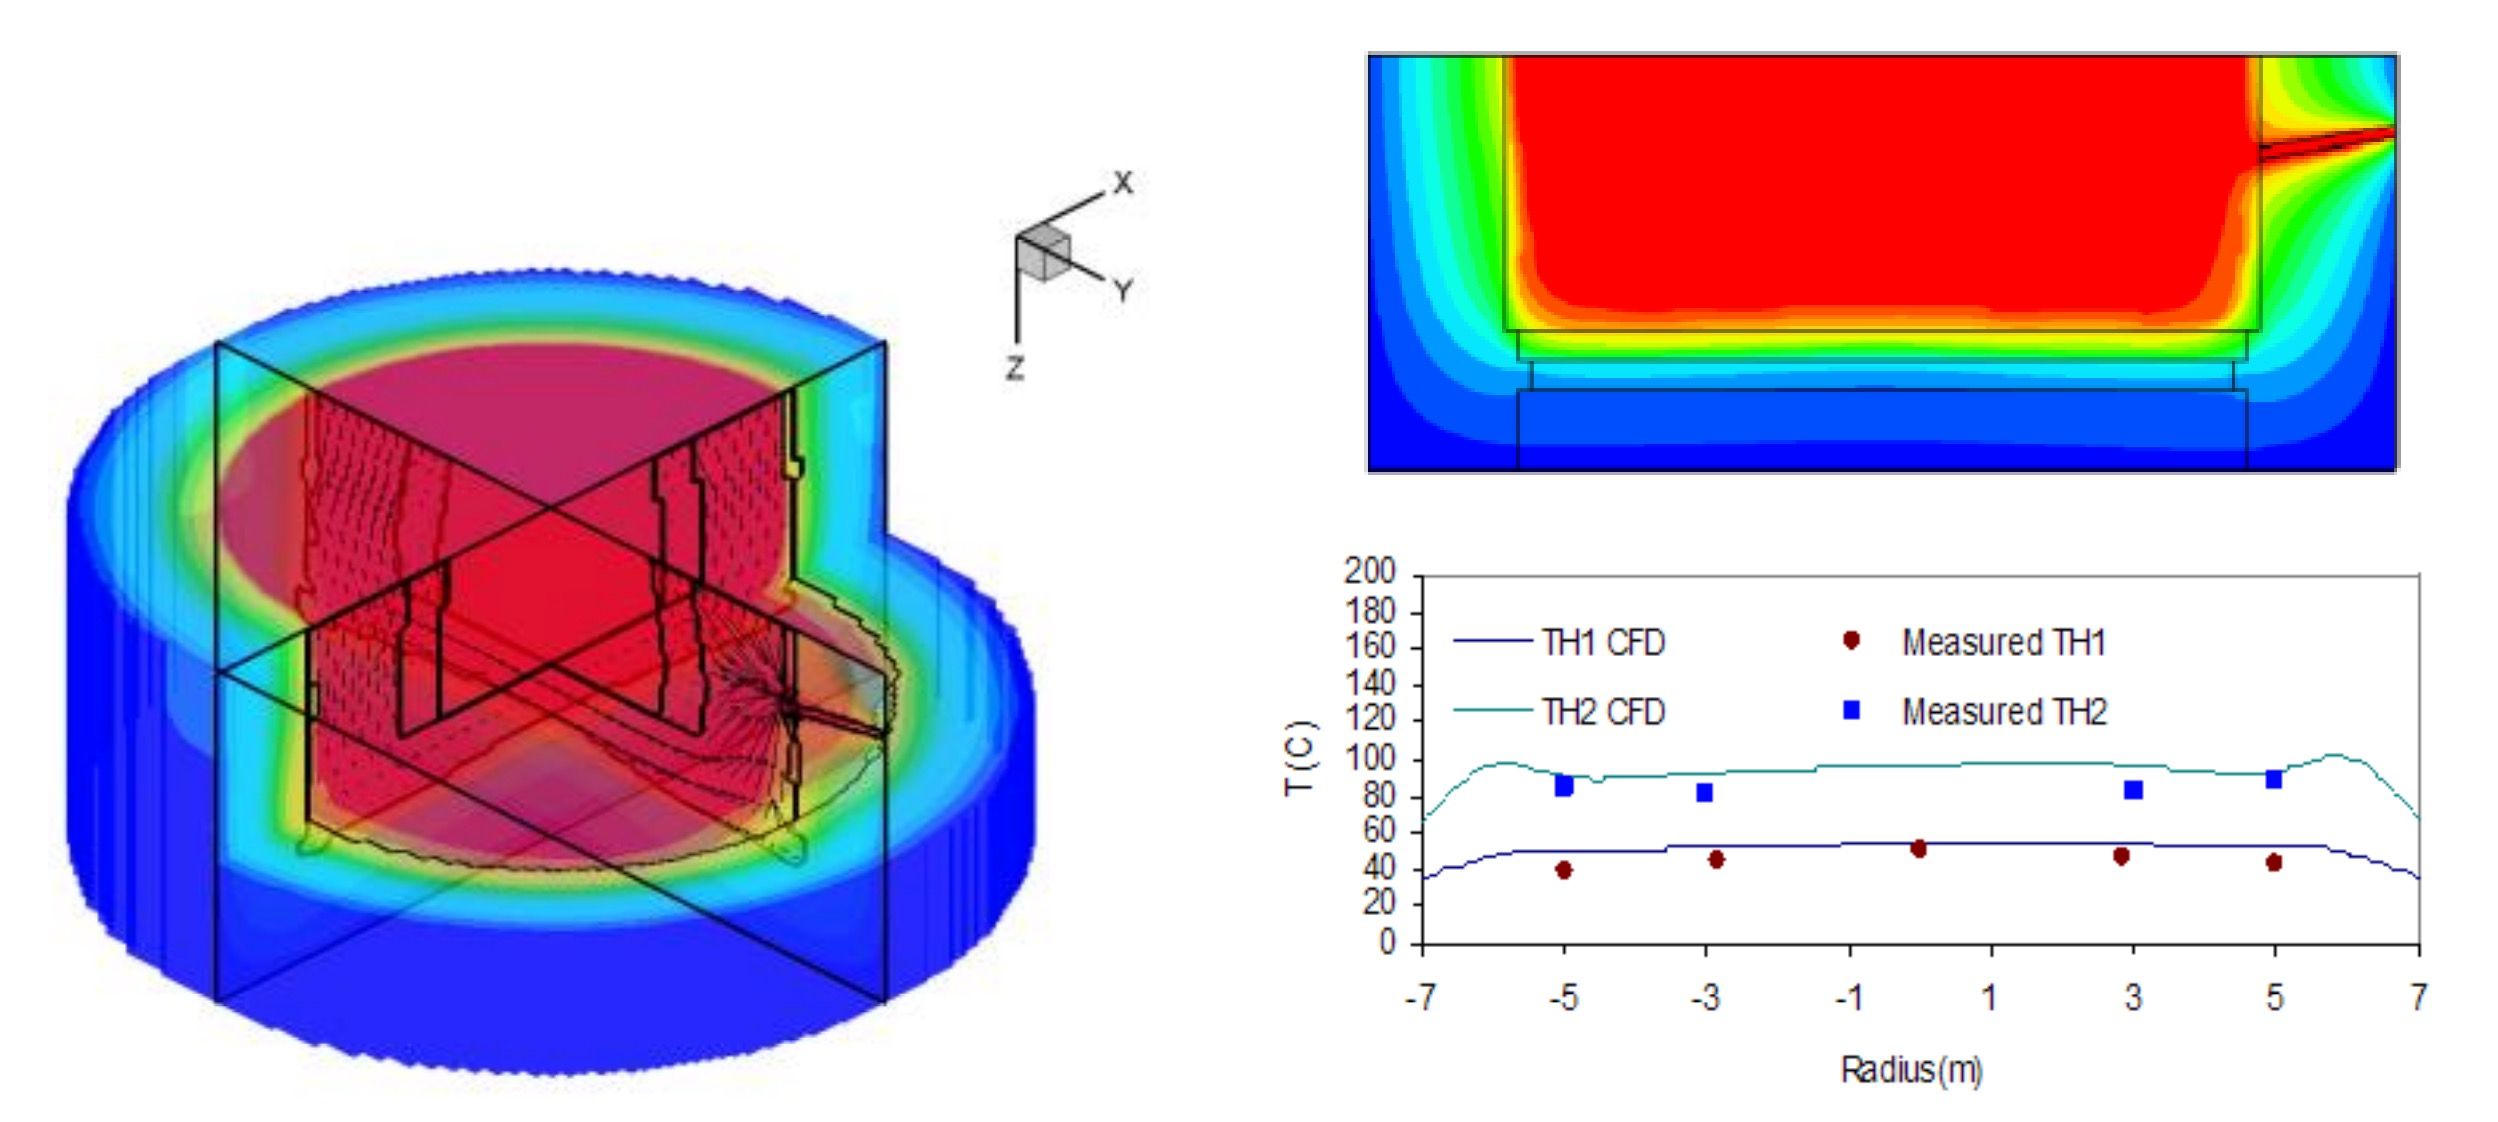
\includegraphics[width=.8\textwidth,angle=0]{blast-furnace-erosion-cfd.jpg}
	\caption{Interactive, educational simulation of basic oxygen steelmaking by steeluniversity.org.}
	\label{o:m6}
\end{figure}

\begin{figure}[h!]
	\centering
	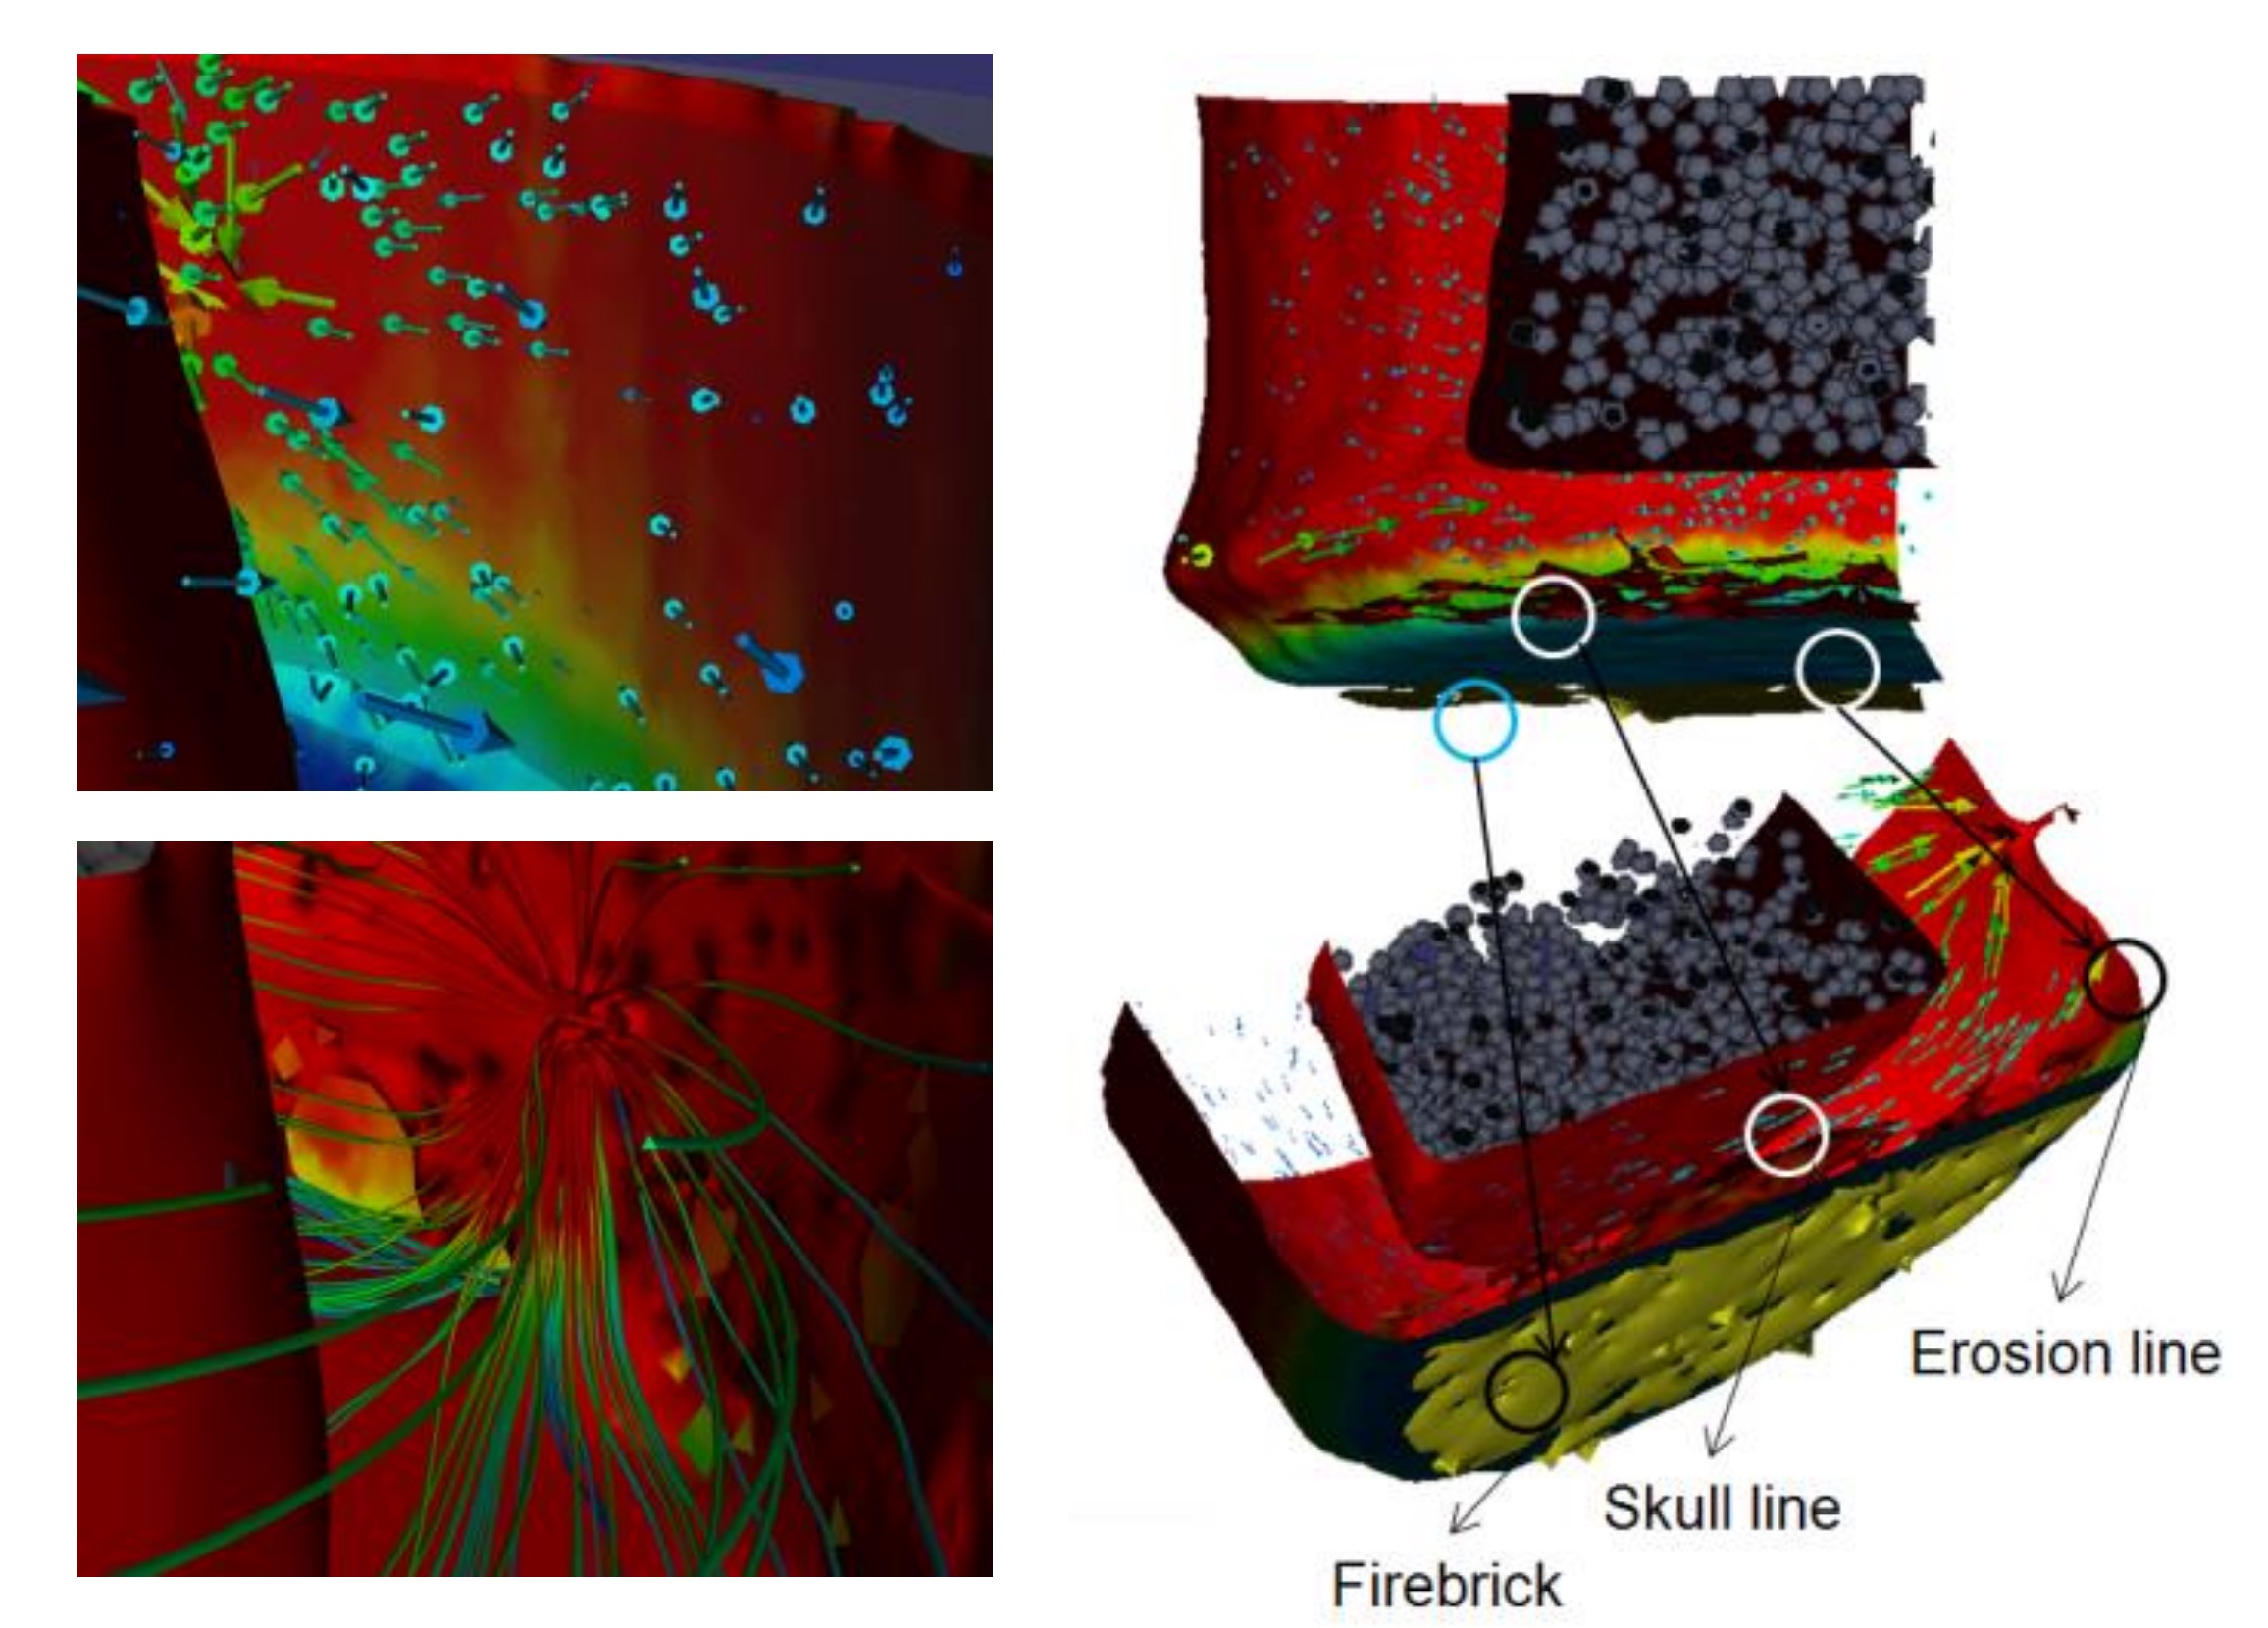
\includegraphics[width=.8\textwidth,angle=0]{blast-furnace-erosion-vr.jpg}
	\caption{Interactive, educational simulation of basic oxygen steelmaking by steeluniversity.org.}
	\label{o:m7}
\end{figure}

The campaign life of a blast furnace is highly dependent on residual thickness of refractory lining in the hearth. The progress of hearth lining erosion is greatly affected by hot metal flow patterns and heat transfer in refractory under different operating
conditions. Thus it is of great importance to monitor the hearth erosion and adjust operating conditions accordingly to prevent further erosion. The difficulty of measurement in the hearth makes computational fluid dynamics (CFD) modeling more
feasible in hearth erosion prediction.

The CFD model has been applied to predict the hearth inner profiles of the actual blast furnace and understand the effects of operation conditions. The results can be used to predict the inner profile of hearth and to provide guidance for protecting the hearth.

Virtual realia shares many of the same characteristics as VR, while in other ways the two experiences differ substantially. Vr displays, for example, simulate the experiences of manipulating a real object but without the need for the immersive environment characteristic of VR. Following the Extent of Presence Metaphor dimension of Milgram and Kishino’s (1994) ‘‘virtuality continuum,’’ Vr is essentially a window-on- the-world with a fixed monoscopic viewpoint; changes in the viewer’s head position do not result in different perspectives of the object. Immersive virtual environments, by comparison, lie at the other end of the spectrum and permit looking around an object by moving one’s head position. Therefore, a fundamental difference between Vr and VR is that the latter is a true 3D representation that may be either viewer or object-centered while the latter is exclusively viewercentered (Kosslyn 1994). In other words, changes in the relative positions of a 2D object’s components result from shifts in the viewer’s perspective. The same may be true for objects viewed in a three dimensional environment, whether real or virtual. However, in such an environment, an object may also appear to change shape (e.g., through foreshortening), not due to an altered position of the viewer, but because the object itself has moved to a different position \citep{Kealy2006}.

Because, sensory breadth contributes more than sensory depth to the experience of presence, it follows that reproduction fidelity is easier to achieve in Vr versus VR, yet more critical to the success of the latter \citep{Kealy2006}.

 the advent of commodity-level virtual reality (VR) hardware has made this technology accessible for meaningful applications. 

 
 Meaningful applications and techniques are being developed to discern how immersive technology benefits visualization. The medical field provides an especially promising context for this development, as medical practitioners require a thorough understanding of specific 3D structures: human anatomy. The most commonly disseminated visualization tools for learning these complex, 3D relationships rely on 2-dimensional (2D) representations. However, when 2D visualizations are used to represent 3D structures, there is a risk of information loss and important interactions between anatomical structures can be absent.
 
 One of In the simulation, users may interact simultaneously with high resolution computed tomography (CT) scans and their corresponding, 3D anatomical structures.

Virtual reality (VR) applications have great potentials for use in education at all levels. VR interfaces have the potentials to complement existing approaches in education. In virtual worlds, learners can be simultaneously provided with three-dimensional representations, multiple perspectives and frames-of-reference, simultaneous visual and auditory feedbacks. With careful de- sign and implementation, these capabilities can be synthesised to create a profound sense of motivation and concentration conducive to mastering complex materials. However, few educational applications have been developed and reported. Shin has reported a desktop VR system for science education in the areas of earth sciences for middle school students (Shin, 2002). VR simulations were developed to teach science concepts such as radiation balance, earthquakes waves, movement of the ocean and earth crust balance. A virtual instrument of a gas chromatograph-mass spectrometer was set up in a web-based environment to train students in instrument operation (Waller \& Foster, 2000). Students learn to operate the virtual instrument via the website outside the laboratory, thus freeing the instrument for use within the laboratory to run meaningful experiments and collect data.

Virtual reality is the use of computers and human-computer interfaces to create the effect of a three-dimensional world containing interactive objects with a strong sense of three-dimensional presence \citep{Bryson1996}.

Immersing the user in the solution, virtual reality reveals the spatially complex structures in computational science in a way that makes them easy to understand and study. But beyond adding a 3D interface, virtual reality also means greater computational complexity \citep{Bryson1996}.


The ability to provide real-time interaction can provide strong depth cues, either through allowing interactive rotations or through the use of head-tracked rendering.

There are, of course, visualization techniques that demand considerable graphics performance, such as isosurfaces and volumetric rendering. In a large data set, a typical isosurface may contain tens of thousands of (logically) disconnected polygons. These polygons are difficult to render within real-time performance constraints. Ways of meeting this problem for isosurfaces include subsampling the surface (potentially masking interesting features), rearranging the polygons so they are optimized for the graphics hardware, hashing the polygon list to replace coplanar neigh- boring polygons with a single polygon, and limiting the spatial extent of the isosurface. Many or all of these techniques may be necessary to achieve real-time performance demands, and even then a limited number of isosurfaces may be practical. Time-intensive methods, such as ray-traced or volumetric rendering, may be impractical in real-time applications.

However, in the section on scientific visualization, we suggested that real-time performance is only one of two requirements of a scientific exploration envi- ronment; the other requirement is a natural, inher- ently three-dimensional, human-conforming interface. By this we mean an interface that is used in as natural a way as possible, that provides as unam- biguous a three-dimensional display as possible, and that requires as little as possible of the user’s atten- tion. This approach contrasts with the current inter- action paradigm in scientific visualization based on text or two-dimensional input through graphical user interfaces and two-dimensional projections of three- dimensional scenes. Conventional interfaces make it difficult to specify positions in three dimensions and do not provide unambiguous display of three-dimen- sional structure.

Virtual reality interfaces attempt to provide the most anthropomorphic interfaces possible. Virtual reality interfaces must include two components: display and user control. 

Scientific visualization makes particular demands on virtual reality displays. The phenomena to be displayed in a scientific visualization application often involve delicate and detailed structure, requiring high-quality, high-resolution full-color displays. A wide field of view is often desirable, because it allows the researcher to view how detailed structures are related to larger, more global phenomena.

Historically, the early attempts at using head-mounted virtual reality technologies started with CRT-based Binocular Omni-Oriented Monitor (BOOM) created by Fakespace Systems Inc. BOOM is a stereoscopic display device with screens and optical system housed in a box that is attached to a multi-link arm. The user looks into the box through two holes, sees the virtual world, and can guide the box to any position within the operational volume of the device. Head tracking is accomplished via sensors in the links of the arm that holds the box.

Another frequently used type of immersive, interactive display technology is projection-screen-based Cave Automatic Virtual Environment (CAVE). These systems consists of 3 to 6 large displays positioned into a room-sized cube around the observer. The walls of a CAVE are typically made up of rear-projection screens, but recently the flat panel displays are commonly used. The floor can be a downward-projection screen, a bottom projected screen or a flat panel display. The projection systems are very high-resolution due to the near distance viewing which requires very small pixel sizes to retain the illusion of reality. The user wears 3D glasses inside the CAVE to see 3D graphics generated by the CAVE. People using the CAVE can see objects apparently floating in the air, and can walk around them, getting a proper view of what they would look like in reality. This is made possible by infrared cameras. Movement of the observer in the CAVE is tracked by the sensors typically attached to the 3D glasses and the video continually adjusts to retain the viewers perspective.

Many universities and engineering companies own and use CAVE systems. Researchers can use these systems to conduct their research topic in a more effective and accessible method. Engineers have found them useful in enhancing of a product development through prototyping and testing phases.

\section{Objectives of the dissertation}
This dissertation thesis deals with design and implementation of 

\section{Methodology}


